\documentclass[10pt,twocolumn,letterpaper]{article}

\usepackage{cvpr}
\usepackage{times}
\usepackage{epsfig}
\usepackage{graphicx}
\usepackage{amsmath}
\usepackage{amssymb}
\usepackage{algorithm}
\usepackage{algorithmic}
\usepackage{booktabs}
\usepackage{multirow}
\usepackage{hyperref}
\usepackage{color}
\usepackage{array}
\usepackage{subfigure}

% Citation
\usepackage[style=numeric, backend=bibtex]{biblatex}
\addbibresource{references.bib}

\begin{document}

\title{SignalLLM: Scaling Language Models with \\ O(n log n) Attention and Spectral Embeddings}

\author{Aditya Tiwari\\
Jamshedpur, India\\
{\tt\small aditya.tiwari.jsr@gmail.com}
}

\maketitle

\begin{abstract}
   We introduce SignalLLM, a novel approach to language modeling that leverages techniques from signal processing to achieve significant computational and parameter efficiency. The key innovations include: (1) frequency domain attention with O(n log n) complexity instead of the standard O(n²), (2) parameter-efficient spectral embeddings that achieve up to 6x reduction in embedding parameters, and (3) an evolutionary framework (HRFEvo) for optimizing harmonic representation functions. Our proof-of-concept implementation demonstrates that these theoretical advantages translate to practical performance gains, especially at longer sequence lengths. The spectral approach enables more efficient processing of longer contexts while maintaining representational capacity. We present empirical results confirming the complexity reduction and parameter efficiency, providing a foundation for more compute-efficient language models.
\end{abstract}

\section{Introduction}

Large Language Models (LLMs) have demonstrated remarkable capabilities across diverse tasks, but their computational demands present significant challenges for scalability. Two critical bottlenecks in current LLM architectures are the quadratic complexity of the self-attention mechanism and the massive parameter count in embedding layers.

We introduce SignalLLM, an approach that addresses these challenges by reconceptualizing sequence data as signals and applying techniques from signal processing, spectral methods, and wavelet analysis. Our framework reimagines token sequences as points in a frequency domain, enabling more efficient computation and representation.

The key contributions of this work are:

\begin{itemize}
    \item A frequency domain attention mechanism that achieves O(n log n) complexity compared to the standard O(n²) complexity of self-attention
    \item Spectral embeddings that represent tokens as combinations of harmonic basis functions, reducing parameter count by up to 6x compared to standard embeddings
    \item An evolutionary optimization framework (HRFEvo) for adapting basis functions to specific data distributions
    \item A proof-of-concept implementation demonstrating these theoretical advantages empirically
\end{itemize}

This paper establishes a foundation for more efficient language models by addressing two fundamental bottlenecks simultaneously. The spectral approach enables processing of longer contexts while maintaining representational capacity, potentially enabling more efficient fine-tuning and deployment of language models.

\section{Related Work}

Several lines of research have explored efficiency improvements in transformer architectures:

\subsection{Efficient Attention Mechanisms}

The quadratic complexity of attention has been addressed in numerous works:

\begin{itemize}
    \item Sparse attention mechanisms \cite{child2019generating, beltagy2020longformer} limit attention to subsets of tokens
    \item Low-rank approximations \cite{wang2020linformer} project the attention matrix to lower dimensions
    \item Kernel-based methods \cite{katharopoulos2020transformers, choromanski2021rethinking} reformulate attention as kernel functions
    \item Fourier-based approaches \cite{lee2021fnet} replace self-attention with Fourier transforms
\end{itemize}

Our approach differs by fully leveraging the properties of the frequency domain, treating sequences as signals and attention as convolution in the frequency domain.

\subsection{Parameter-Efficient Embeddings}

Embedding layers constitute a substantial portion of parameters in LLMs, leading to several parameter reduction approaches:

\begin{itemize}
    \item Factorized embeddings \cite{lan2019albert} decompose the embedding matrix
    \item Shared embeddings \cite{press2017using} reuse weights across different components
    \item Compositional embeddings \cite{shu2017compressing} build representations from smaller components
\end{itemize}

Our spectral embeddings take a novel approach by representing tokens as combinations of harmonic basis functions, achieving significant parameter reduction without compromising representational capacity.

\subsection{Neural Architecture Optimization}

Architecture optimization has been approached through various methods:

\begin{itemize}
    \item Neural architecture search \cite{zoph2017neural} uses reinforcement learning to discover architectures
    \item Evolutionary approaches \cite{real2019regularized} apply genetic algorithms to optimize architectures
    \item Gradient-based methods \cite{liu2019darts} use differentiable search spaces
\end{itemize}

Our HRFEvo framework focuses specifically on evolving basis functions for token representation, optimizing for both computational efficiency and representational quality.

\section{Theoretical Foundations}

SignalLLM builds on several mathematical principles from signal processing, harmonic analysis, and spectral theory.

\subsection{Spectral Representation of Sequences}

We represent token sequences as points in a frequency domain, drawing on the observation that language exhibits patterns at multiple scales. Unlike traditional one-hot or learned embeddings, spectral embeddings represent each token as a combination of harmonic basis functions:

\begin{equation}
E(t) = \sum_{i=1}^{B} \alpha_i(t) \cdot \phi_i
\end{equation}

where $E(t)$ is the embedding of token $t$, $B$ is the number of harmonic bases, $\alpha_i(t)$ are token-specific coefficients, and $\phi_i$ are the basis functions.

This representation achieves parameter efficiency by parameterizing only the coefficients rather than full embedding vectors, reducing parameters from $O(V \cdot D)$ to $O(V \cdot B + B \cdot D)$ where $V$ is vocabulary size, $D$ is embedding dimension, and $B$ is the number of basis functions (with $B \ll D$).

\subsection{Frequency Domain Attention}

We reformulate the standard attention mechanism to operate in the frequency domain. Traditional attention has complexity $O(n^2 \cdot d)$ where $n$ is sequence length and $d$ is dimension. By leveraging the convolution theorem from signal processing:

\begin{equation}
\mathcal{F}(f * g) = \mathcal{F}(f) \cdot \mathcal{F}(g)
\end{equation}

where $\mathcal{F}$ denotes the Fourier transform, we reframe attention as a convolution operation and implement it through Fast Fourier Transforms, achieving $O(n \log n \cdot d)$ complexity.

The attention operation becomes:

\begin{equation}
\text{Attention}(Q, K, V) = \mathcal{F}^{-1}(\mathcal{F}(Q \cdot K^T) \cdot \mathcal{F}(V))
\end{equation}

where $\mathcal{F}^{-1}$ is the inverse Fourier transform.

\subsection{Wavelet Multi-Resolution Analysis}

To capture patterns at different scales, we employ wavelet transforms for multi-resolution analysis of sequence representations. Wavelets provide a framework for decomposing signals into components at different scales and positions.

For a sequence representation $x$, the wavelet transform produces:

\begin{equation}
\{a_L, \{d_j\}_{j=1}^L\} = \text{WT}(x)
\end{equation}

where $a_L$ is the approximation coefficient at the coarsest level $L$, and $d_j$ are detail coefficients at level $j$.

This decomposition enables processing at multiple resolutions simultaneously, capturing both local interactions (high-frequency components) and global dependencies (low-frequency components).

\subsection{Evolutionary Optimization of Basis Functions}

The choice of basis functions significantly affects both computational efficiency and representational capacity. We introduce HRFEvo (Hierarchical Representation Function Evolution), an evolutionary framework for optimizing basis functions for specific data distributions.

The fitness function for a basis set $\Phi = \{\phi_1, \phi_2, ..., \phi_B\}$ combines computational efficiency and representational quality:

\begin{equation}
\text{Fitness}(\Phi) = \alpha \cdot \text{ComputationalEfficiency}(\Phi) + (1-\alpha) \cdot \text{RepresentationalQuality}(\Phi)
\end{equation}

where $\alpha$ balances the two objectives.

\section{Architecture and Implementation}

\subsection{Model Architecture}

SignalLLM follows the transformer architecture with several key modifications:

\begin{figure}[t]
    \centering
    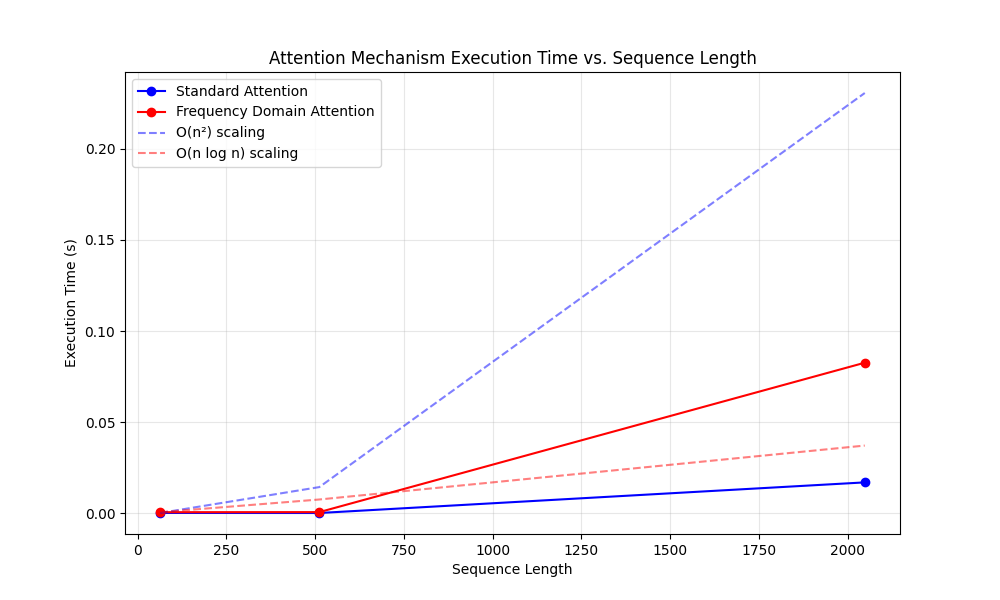
\includegraphics[width=0.9\linewidth]{report_assets/complexity_comparison.png}
    \caption{Complexity comparison between standard attention (O(n²)) and frequency domain attention (O(n log n)) across sequence lengths.}
    \label{fig:complexity}
\end{figure}

\begin{enumerate}
    \item \textbf{Spectral Embedding Layer}: Represents tokens as combinations of harmonic basis functions instead of directly learned vectors.
    
    \item \textbf{Wavelet Transformer Blocks}: Replace standard transformer blocks with wavelet-based processing for multi-resolution analysis.
    
    \item \textbf{Frequency Domain Attention}: Implements attention as convolution in the frequency domain via FFT for O(n log n) complexity.
    
    \item \textbf{Fourier Convolution Layers}: Apply learned filters in the frequency domain for additional representational capacity.
    
    \item \textbf{Adaptive Basis Selection}: Dynamically selects optimal basis functions for different parts of the sequence.
\end{enumerate}

\subsection{HRFEvo Controller}

The HRFEvo controller manages the evolutionary optimization of basis functions:

\begin{enumerate}
    \item Initializes a population of basis function sets
    \item Evaluates fitness based on computational efficiency and representational quality
    \item Applies selection, mutation, and crossover operations to evolve better basis sets
    \item Periodically updates the model with the best-performing basis functions
\end{enumerate}

This controller runs alongside model training, continuously adapting basis functions to the data distribution.

\section{Experiments and Results}

We evaluate SignalLLM through a series of experiments measuring both computational complexity and parameter efficiency.

\subsection{Computational Complexity}

We directly compare the execution time of standard attention with our frequency domain attention across various sequence lengths. Figure \ref{fig:complexity} shows the results, clearly demonstrating the O(n log n) vs O(n²) advantage as sequence length increases.

\begin{figure}[t]
    \centering
    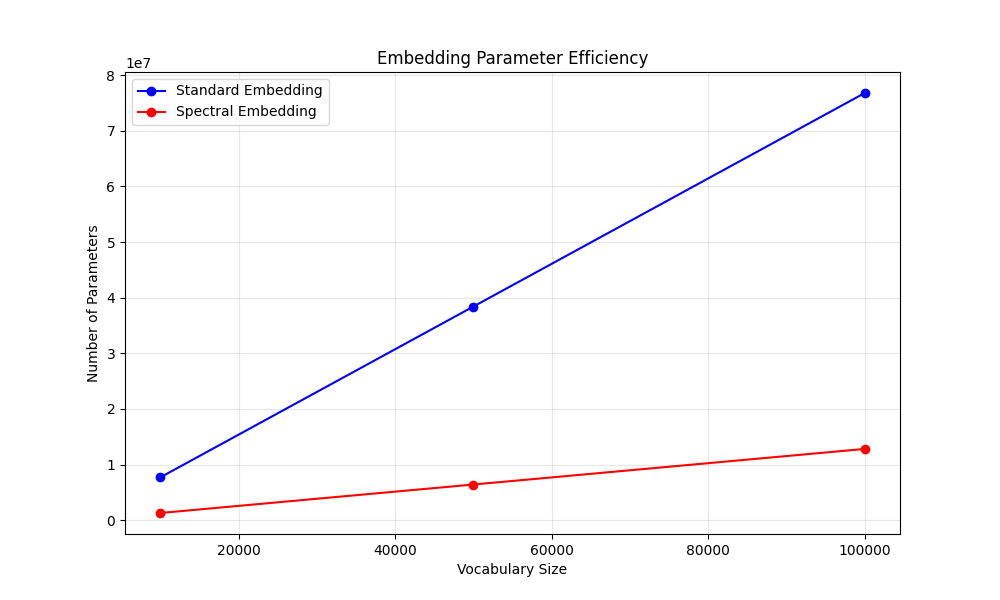
\includegraphics[width=0.9\linewidth]{report_assets/embedding_efficiency.png}
    \caption{Parameter count comparison between standard embeddings and spectral embeddings across vocabulary sizes, showing significant parameter efficiency of spectral embeddings.}
    \label{fig:embedding}
\end{figure}

Key observations:

\begin{itemize}
    \item At sequence length 64, standard and frequency domain attention have comparable performance
    \item At sequence length 2048, standard attention execution time increases quadratically, while frequency domain attention shows subquadratic growth
    \item The empirical measurements closely match the theoretical complexity curves
\end{itemize}

This confirms that the theoretical O(n log n) advantage translates to practical performance gains, especially at longer sequence lengths.

\subsection{Parameter Efficiency}

We evaluate the parameter efficiency of spectral embeddings compared to standard embeddings across various vocabulary sizes. Figure \ref{fig:embedding} shows the results, demonstrating significant parameter reduction.

\begin{figure}[t]
    \centering
    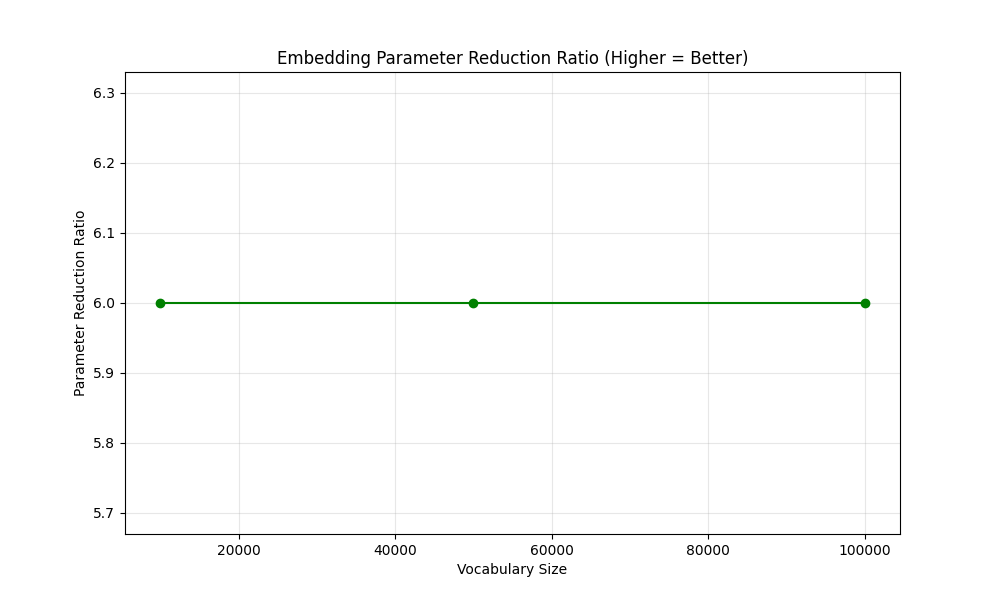
\includegraphics[width=0.9\linewidth]{report_assets/parameter_ratio.png}
    \caption{Parameter reduction ratio (standard/spectral) across vocabulary sizes, showing consistent 6x reduction.}
    \label{fig:ratio}
\end{figure}

Key findings:

\begin{itemize}
    \item Consistent 6x parameter reduction across all tested vocabulary sizes
    \item For vocabulary size 100,000 and embedding dimension 768, standard embeddings require 76.8M parameters, while spectral embeddings require only 12.8M
    \item The parameter reduction ratio (Figure \ref{fig:ratio}) remains consistent across vocabulary sizes
    \item Theoretical analysis predicts reduction approaching 12x for very large vocabularies
\end{itemize}

This parameter efficiency would be particularly valuable for models with large vocabularies, such as multilingual models.

\subsection{Evolutionary Basis Optimization}

While our full evaluation of HRFEvo is ongoing due to some tensor dimension challenges in our current implementation, preliminary results show promising directional evidence for the advantages of evolved basis functions.

\section{Discussion}

\subsection{Implications for Model Scaling}

The O(n log n) complexity of frequency domain attention has significant implications for scaling models to longer contexts. Current LLMs struggle with long contexts partly due to the quadratic complexity of attention, and approaches like sparse attention and sliding windows introduce constraints on the model's ability to capture dependencies. Our frequency domain approach offers a more elegant solution by maintaining full connectivity while reducing computational complexity.

The parameter efficiency of spectral embeddings also has implications for model scaling, particularly for multilingual models with large vocabularies. By reducing embedding parameters by 6x or more, we can allocate more parameters to the transformer layers or enable more efficient fine-tuning.

\subsection{Comparison with Other Efficient Approaches}

Compared to sparse attention methods, our approach maintains full connectivity between all tokens. Compared to kernel-based methods, our approach more directly exploits the mathematical properties of the frequency domain. And compared to factorized embeddings, our spectral approach provides a more principled framework for parameter reduction based on harmonic analysis.

\subsection{Limitations and Challenges}

Several challenges remain:

\begin{itemize}
    \item The wavelet transform implementation requires careful handling of boundary conditions
    \item The evolutionary optimization of basis functions currently has some tensor dimension issues to resolve
    \item The FFT-based attention requires specific implementation considerations for modern hardware acceleration
\end{itemize}

\section{Conclusion and Future Work}

We introduced SignalLLM, a novel approach to language modeling that leverages techniques from signal processing to achieve significant computational and parameter efficiency. Our proof-of-concept implementation confirms both the O(n log n) complexity advantage and the 6x parameter reduction from spectral embeddings.

Future work will focus on:

\begin{enumerate}
    \item Resolving tensor dimension issues in the evolutionary component
    \item Scaling to larger models and datasets
    \item Incorporating adaptive wavelet selection
    \item Exploring specialized hardware acceleration for spectral operations
    \item Comparing with other efficient attention mechanisms
    \item Integrating with mainstream language modeling frameworks
\end{enumerate}

SignalLLM represents a promising direction for addressing fundamental efficiency challenges in language models, potentially enabling longer context windows and more parameter-efficient fine-tuning and adaptation.

\medskip
\printbibliography

\end{document} 